
%(BEGIN_QUESTION)
% Copyright 2010, Tony R. Kuphaldt, released under the Creative Commons Attribution License (v 1.0)
% This means you may do almost anything with this work of mine, so long as you give me proper credit

The rotational equivalent of {\it force} is something called {\it torque}.  The following diagram shows its physical definition in the context of a rope exerting force on the circumference of a pulley:

$$\includegraphics[width=15.5cm]{i01403x03.eps}$$

Mathematically, torque is the product of the force vector and the radius vector perpendicular to the force (called the ``moment arm''):

$$\vec \tau = \vec r \times \vec F$$

Based on this formula, determine the proper unit of measurement for torque, given force in {\it pounds} and radius in {\it feet}.

\vskip 10pt

Next, calculate the amount of torque applied to the bolt head by the wrench, assuming the force measures 82 ounces and the length of the moment arm is 17 inches:

$$\includegraphics[width=15.5cm]{i01403x01.eps}$$

\filbreak

\vskip 20pt \vbox{\hrule \hbox{\strut \vrule{} {\bf Suggestions for Socratic discussion} \vrule} \hrule}

\begin{itemize}
\item{} An important detail to note is that although the formulae for calculating torque involves the multiplication of {\it pounds} of force and {\it feet} of distance just like the formula for work ($W = Fx$), torque in pound-feet is definitely not the same thing as work in foot-pounds.  Give a practical example illustrating how torque and work cannot be the same quantity despite bearing very similar units of measurement.
\end{itemize}

\underbar{file i01403}
%(END_QUESTION)





%(BEGIN_ANSWER)

$\tau$ = 7.26 lb-ft

%(END_ANSWER)





%(BEGIN_NOTES)

\noindent
If $F$ = 82 oz and $r$ = 17 in:

$\tau$ = 1394 oz-in (7.26 lb-ft) 

\vskip 10pt

It should be noted that while torque is the product of force and distance, it is not the same as {\it work}, which is also a product of force and distance:

$$W = \vec F \cdot \vec d$$

Torque is a cross-product, while work is a dot-product.  Cross-products are always vectors, while dot products are always scalars.  This makes intuitive sense, too: torque always exists along an {\it axis of rotation}, which necessarily has a direction.  Work has no intrinsic direction, but is a simple scalar quantity.

In honor of this distinction, the unit of measurement for torque in the English system is lb-ft, while the unit of measurement for work is the ft-lb.  In the metric system, newton-meters is used for both torque and work, which is unfortunate.

%INDEX% Physics, torque: axis of rotation
%INDEX% Physics, torque: calculation problem
%INDEX% Physics, torque: line of action
%INDEX% Physics, torque: moment arm

%(END_NOTES)


